\section{Open Question}
\label{sec:open}
\subsection{Research question}
Is the scientific community on Bluesky organized into topical echo chambers? Concretely:
\begin{itemize}\itemsep0pt
    \item do the network communities correspond to coherent discussion topics;
    \item are connected accounts more topically similar than unconnected ones (topical homophily); and
    \item how does that homophily evolve across successive account generations?
\end{itemize}

\subsection{Method}
SNA is combined with text mining, exploiting the post layer collected during crawling. Each node is turned into a document by concatenating its sampled posts ($\sim$271k posts over $14{,}598$ active accounts); documents are vectorized with TF-IDF (3{,}000 terms, English plus platform stop-words). Four analyses follow.
\begin{enumerate}
\item The top TF-IDF terms per Louvain community label its topic. \item To quantify how far a follow-community is a topic, the documents are independently clustered into topical groups (KMeans, one cluster per Louvain community) and the two partitions are compared via Normalized Mutual Information (NMI) and the Adjusted Rand Index (ARI).
\item Topical homophily is measured as the mean cosine similarity between topic vectors, contrasting same vs different community pairs and real edges vs non-edges, with a one-sided Mann--Whitney test; the edge comparison is also checked against a degree-preserving configuration-model null (script \texttt{open\_question\_null.py}).
\item The echo chamber is tracked over time by splitting accounts into creation-year cohorts (2023/2024/2025) and measuring, within each, the topical homophily of the internal follow edges (edge similarity relative to random within-cohort pairs).
\end{enumerate}

\subsection{Results}
The seven largest communities map onto sharply distinct disciplines (Table~\ref{tab:topics}): politics/news (trump, news, iran), climate/energy (climate, energy, ocean), chemistry/biology (nature, cell, chemistry), neuroscience (brain, neuroscience), conservation/ecology (species, biodiversity, marine), public health (health, vaccine, ebola) and space (nasa, space, moon). This structure--topic correspondence is only partial, however: a purely text-based clustering agrees with the Louvain partition at $\mathrm{NMI}=0.23$ and $\mathrm{ARI}=0.13$, clearly above chance yet far from identical, so following and talking are related but not interchangeable. Topical cohesion also varies by community (Table~\ref{tab:topics}, last column): the tightest echo chambers are the specialised neuroscience ($0.069$) and conservation ($0.068$) clusters, the loosest the cross-cutting politics/news ($0.053$) and space ($0.056$) ones. Connected accounts are markedly more similar: same-community pairs are $1.38\times$ more topically similar than cross-community pairs ($0.060$ vs $0.043$), and the endpoints of real follow edges are $1.83\times$ more similar than random non-edges ($0.086$ vs $0.047$). Both gaps are highly significant (one-sided Mann--Whitney $U$, $p<10^{-80}$ for communities and $p<10^{-200}$ for edges), and the full distributions (Figure~\ref{fig:homophily}) show the same ordering. The effect is not an artifact of the vectorization: shrinking or enlarging the TF-IDF vocabulary from $3{,}000$ to $1{,}500$ or $5{,}000$ terms leaves both ratios essentially unchanged ($1.34$--$1.36\times$ for communities and $1.72$--$1.90\times$ for edges). A stricter, degree-preserving control points the same way: compared against a configuration-model null whose pairs are drawn in proportion to node degree (reproducing the endpoints' degree but scrambling who links to whom), real follow edges remain $1.55\times$ more topically similar (one-sided Mann--Whitney $p<10^{-140}$), so the homophily is not merely an effect of the hubs' high degree. Crucially, the edge-level comparison is model-free: topic vectors are built only from post text and the two endpoints of a follow tie are compared directly, with no reference to the follow graph or to the Louvain labels. The $1.83\times$ gap is therefore not an artifact of how the communities were defined; structure (who follows whom) and content (what accounts write) are measured independently and only then correlated.

\begin{table}[h]
  \centering\footnotesize
  \setlength{\tabcolsep}{4pt}
  \caption{Representative TF-IDF terms and intra-community topical cohesion (mean pairwise post-content cosine similarity) of the seven largest Louvain communities.}
  \label{tab:topics}
  \begin{tabular}{llc}
    \toprule
    Community (topic) & Top TF-IDF terms & Cohesion \\
    \midrule
    politics/news        & trump, news, iran             & 0.053 \\
    climate/energy       & climate, energy, ocean        & 0.064 \\
    chemistry/biology    & nature, cell, chemistry       & 0.066 \\
    neuroscience         & brain, neuroscience           & 0.069 \\
    conservation/ecology & species, marine, biodiversity & 0.068 \\
    public health        & health, vaccine, ebola        & 0.067 \\
    space                & nasa, space, moon             & 0.056 \\
    \bottomrule
  \end{tabular}
\end{table}

\begin{figure}[h]
  \centering
  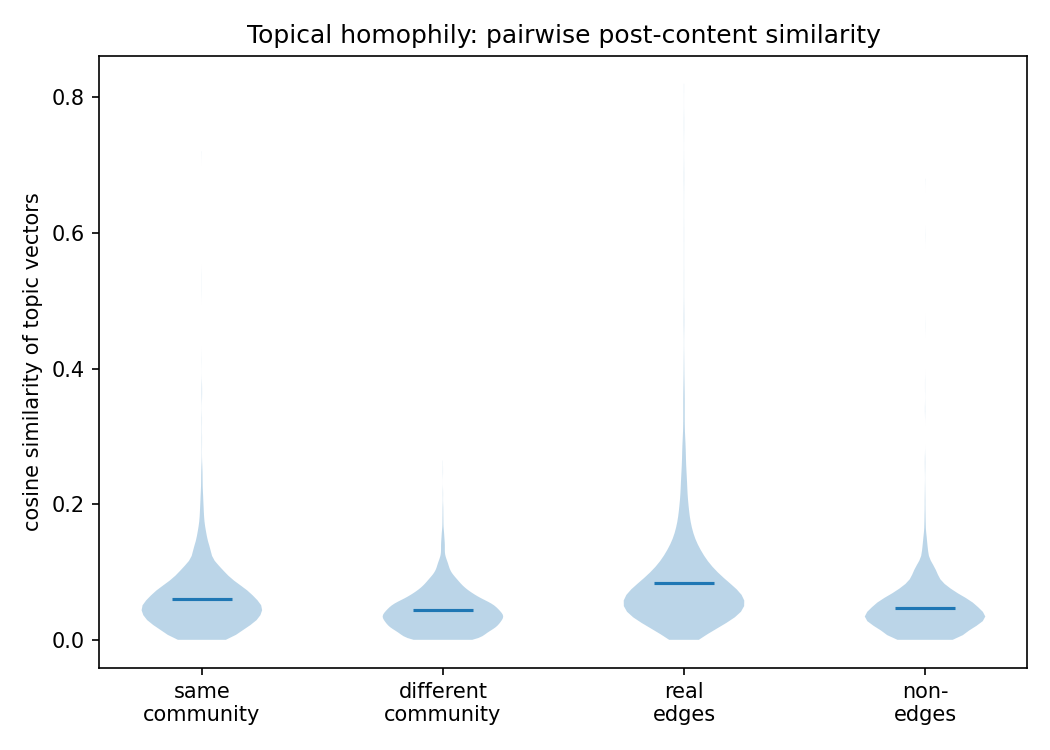
\includegraphics[width=\linewidth]{figures/open_question_homophily.png}
  \caption{Distributions of pairwise topic-vector cosine similarity (means marked): same vs different-community pairs, and real-edge vs non-edge endpoints}
  \label{fig:homophily}
\end{figure}

\subsection{Tracking the echo chamber over time}
Measuring edge homophily separately within each account-creation cohort reveals a clear trend (Figure~\ref{fig:oq-time}): the internal follow edges of the 2023 founding wave are $1.62\times$ more topically homophilous than random within-cohort pairs, but the ratio climbs to $2.33\times$ for the 2024 cohort and $3.52\times$ for the 2025 one. Each new generation of accounts thus enters an increasingly topic-segregated neighborhood: the echo chambers are tightening over time as the community matures.

\begin{figure}[h]
  \centering
  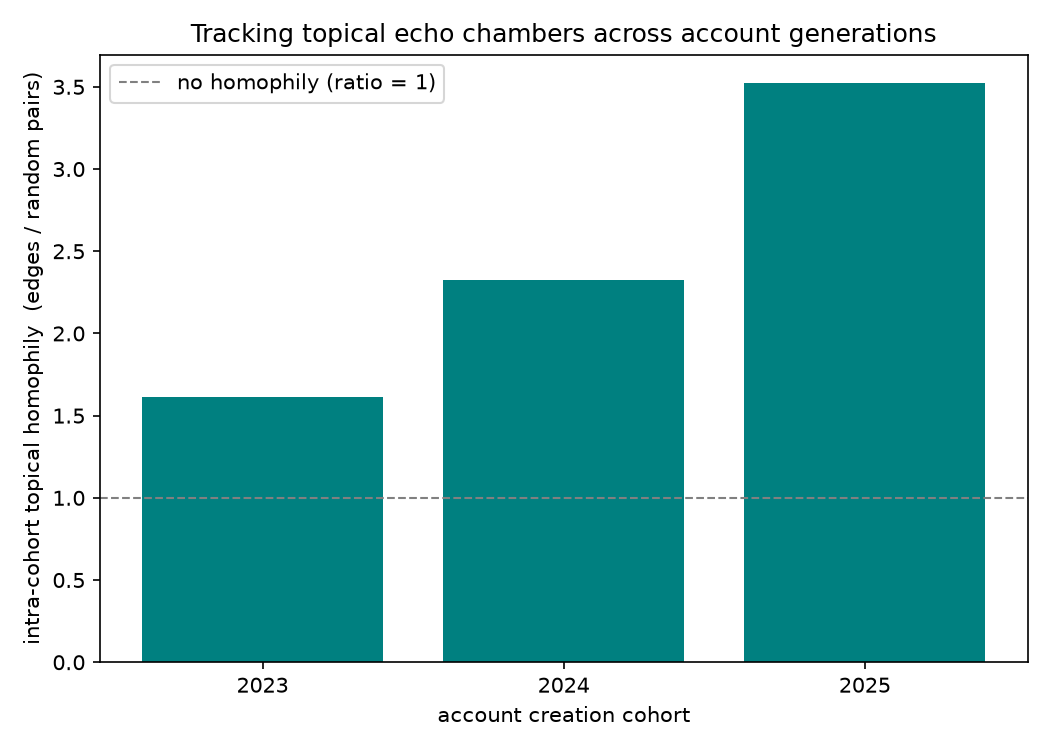
\includegraphics[width=\linewidth]{figures/open_question_temporal.png}
  \caption{Topical homophily of intra-cohort follow edges (edge vs random within-cohort pairs) by account-creation cohort: echo chambers tighten for more recent generations}
  \label{fig:oq-time}
\end{figure}

\subsection{Interpretation}
The measures point the same way: the follow structure aligns with what accounts talk about (people preferentially follow others discussing similar topics) and communities behave as topical clusters. But the partial NMI/ARI and the moderate homophily ratios describe permeable, overlapping chambers, not sealed ones, in line with the cross-cutting role of the journalistic and political accounts seen in Section~\ref{sec:analysis}. The temporal trend qualifies this. Although the community as a whole is permeable, each newer generation of accounts settles into a more topic-segregated neighborhood, so the chambers, while still overlapping, are tightening as the platform matures.

\section{Discussion}
\label{sec:discussion}
The five parts reinforce one another. The structural findings of Section~\ref{sec:analysis}, a heavy-tailed degree distribution and, above all, a clustering coefficient an order of magnitude above the ER baseline, are more than descriptive statistics: they are the topological trace of the community organization that Section~\ref{sec:cd} resolves into recognizable academic disciplines. The same excess of triangles that makes the network non-random is what lets Louvain and Infomap recover meaningful partitions, and what the open question (Section~\ref{sec:open}) explains semantically: accounts cluster because they talk about and follow others on the same topics.

Two themes recur. The first is that the community is cohesive but permeable. Topical homophily is clear though moderate ($1.8\times$), and the most central nodes are not the pure science accounts one might expect: they are platform, journalistic and political hubs (\texttt{bsky.app}, \texttt{nytimes.com}, \texttt{aoc}) that bridge otherwise separate disciplines. The ``echo chambers'' are real, but they overlap. The second theme is that structure governs dynamics. On such a dense graph the epidemic models saturate almost regardless of topology. The custom coordination cascade is more selective: which nodes seed a behavior matters much more than how many (hubs sustain global cascades at $4$--$5\times$ higher thresholds), and the communities detected in Section~\ref{sec:cd} act as diffusion barriers once coordination becomes even slightly homophilous. So the community structure does more than describe the network: it shapes how information and behavior actually spread through the scientific community.

\section{Conclusions}
A 15{,}000-node follow network of the Bluesky scientific community was built and analyzed. The network is small-world and approximately scale-free, with a clustering coefficient far above ER/BA baselines, revealing a strong community structure that Louvain and Infomap resolve into interpretable academic disciplines. Link prediction confirms that local, neighborhood-based heuristics (Adamic--Adar, $21.4\times$ better than random) outperform popularity-based ones, while diffusion simulations, on such a dense graph, saturate almost identically across real and synthetic topologies, the real network even peaking marginally lower due to its redundant intra-community edges. Finally, the open question provides evidence of moderate but tightening topical echo chambers: connected accounts are $1.8\times$ more topically similar than random pairs, follow-communities align with text-topics only partially ($\mathrm{NMI}=0.23$), and intra-cohort homophily rises from $1.6\times$ for the 2023 generation to $3.5\times$ for the 2025 one.

\subsection{Limitations}
The sample reflects the seeds' neighborhood, follow lists are truncated, and posts are a per-account sample; results should be read as characterizing the crawled community, not the whole platform.
